\chapter{Análisis Inicial de los datos.}
Previamente al diseño de la solución, se decidió realizar un análisis de los datos de entrenamiento tal que se pueda determinar sus características y formas en las que pueden ser aprovechadas.

En principio podemos decir que contamos con 42000 imágenes de 28 píxeles de ancho por 28 píxeles de alto. Cada una esta ligada a una clase de entre 10 que pueden ser 0,1,...,9. 

En la Tabla 1.1 se puede observar el porcentaje de imágenes de cada una de las clases que existen en el set de entrenamiento. Se puede decir entonces que los datos están bien balanceados.

\begin{table}[htp]
  \caption{Porcentaje de imágenes de cada una de las clases en el train}
  \label{porc}

  \begin{center}
    \begin{tabular}{|c|c|c|c|c|c|c|c|c|c|c|}
    \hline
      Clase&0&1&2&3&4&5&6&7&8&9 \\
    \hline
      Porcentaje&9.83&11.15&9.94&10.35&9.69&9.03&9.85&10.47&9.67&9.97 \\
    \hline
    \end{tabular}
  \end{center}
\end{table}

Por otro lado si realizamos un promedio de todas las imágenes y observamos los valores obtenidos, daremos cuenta de que existen atributos cuyo valor es 0 en todos los registros. Esto nos da pie a pensar de que podríamos llegar a prescindir de algunos atributos, reduciendo así el costo computacional que requerirá procesar todos estos datos.
\begin{figure}[htp]
  \begin{center}
    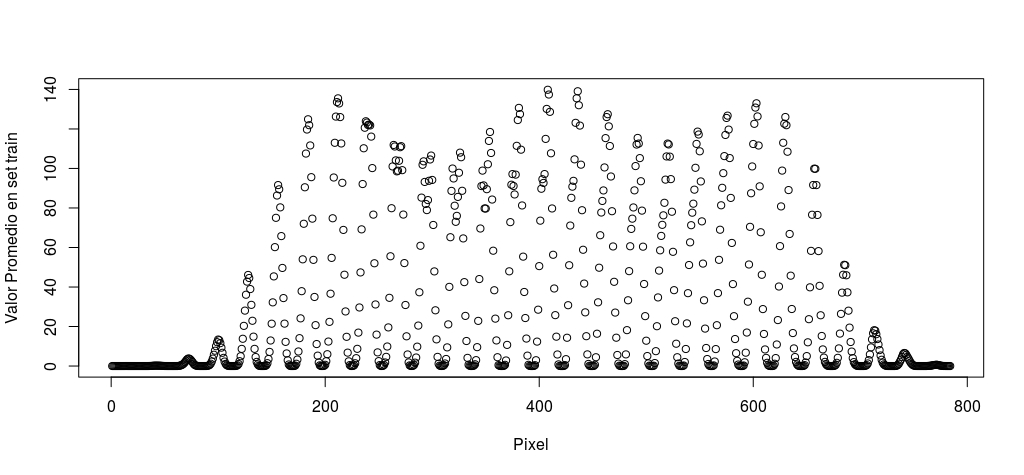
\includegraphics[width=15cm]{Rplot.jpeg}
    \caption{Valores promedio de cada atributo en el set Train}
    \label{plot1}
  \end{center}
\end{figure}

Antes de modificar de alguna forma el set de entrenamiento, analizamos los valores promedio de los atributos de los registros que se encuentran el set de test y sus resultados fueron los siguientes. Figura \ref{plot2}
\begin{figure}[htp]
  \begin{center}
    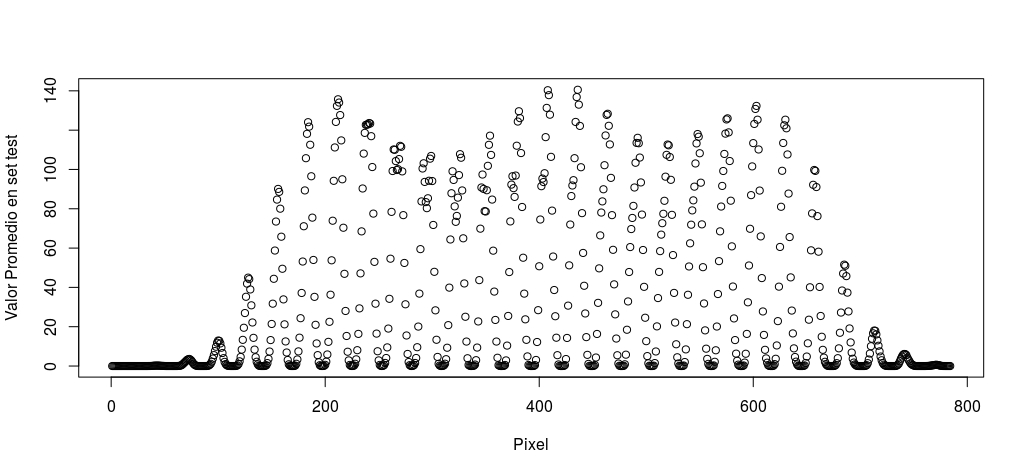
\includegraphics[width=15cm]{Rplot01.jpeg}
    \caption{Valores promedio de cada atributo en el set Test}
    \label{plot2}
  \end{center}
\end{figure}
